%%%%%%%%%%%%%%%%%%%%%%%%%%%%%%%%%%%%%%%%%
% This template has been downloaded from:
% http://www.LaTeXTemplates.com
%
% Original author:
% WikiBooks (http://en.wikibooks.org/wiki/LaTeX/Title_Creation)
%%%%%%%%%%%%%%%%%%%%%%%%%%%%%%%%%%%%%%%%%
%\title{Title page with logo}
%--------------------------------------------------------------
%	PACKAGES AND OTHER DOCUMENT CONFIGURATIONS
%-------------------------------------------------------------

\documentclass[12pt]{article}
\usepackage[english]{babel}
\usepackage[utf8x]{inputenc}
\usepackage{amsmath}
\usepackage{graphicx}
\usepackage[colorinlistoftodos]{todonotes}
\usepackage{floatrow} 
\newfloatcommand{capbtabbox}{table}[][\FBwidth]

\usepackage{fancyhdr} % Required for custom headers
\usepackage{lastpage} % Required to determine the last page for the footer
\usepackage{extramarks} % Required for headers and footers
\usepackage{lipsum} % Used for inserting dummy 'Lorem ipsum' text into the template
\usepackage{bm}
\usepackage{float}
\usepackage{mathtools}
\usepackage{enumerate}
\usepackage{amssymb}
\usepackage{booktabs}
\usepackage{subcaption}
\usepackage{caption}
\usepackage{graphicx}
\usepackage{enumerate}
\usepackage{multirow}


% Margins
\topmargin=-0.45in
\evensidemargin=0in
\oddsidemargin=0in
\textwidth=6.5in
\textheight=9.0in
\headsep=0.25in 
\linespread{1.1} % Line spacing

% Set up the header and footer
\pagestyle{fancy}
\lhead{}
\chead{Spam Email Classification} % Top center header
\rhead{\firstxmark} % Top right header
\lfoot{\lastxmark} % Bottom left footer
\cfoot{} % Bottom center footer
\rfoot{Page\ \thepage\ of\ \pageref{LastPage}} % Bottom right footer
\renewcommand\headrulewidth{0.4pt} % Size of the header rule
\renewcommand\footrulewidth{0.4pt} % Size of the footer rule

\setlength\parindent{0pt} % Removes all indentation from paragraphs



\begin{document}

\begin{titlepage}

\newcommand{\HRule}{\rule{\linewidth}{0.5mm}} % Defines a new command for the horizontal lines, change thickness here

\center % Center everything on the page
 
%--------------------------------------------------------------
%	HEADING SECTIONS
%--------------------------------------------------------------

\textsc{\LARGE University of California Davis }\\[0.3cm] 
\textsc{\Large Department of Statistics}\\[0.5cm] 
 % Minor heading such as course title

%--------------------------------------------------------------
%	TITLE SECTION
%--------------------------------------------------------------

\HRule \\[0.4cm]
{ \huge \bfseries Machine Learning\\  (STA-208)}\\[0.03cm]
\HRule \\[1.5cm]

\hfill \break \hfill \break \hfill \break
\hfill \break \hfill \break \hfill \break 
\hfill \break \hfill \break \hfill \break
\hfill \break

{\large Ying-Chen Chou \\ Chia-Hui Shen \\Jiahui Tan\\ Pei-Ying Ling}\\


\includegraphics[width=4cm]{logo.png}\\[1cm] 
 
%--------------------------------------------------------------

\vfill % Fill the rest of the page with whitespace

\end{titlepage}

\newpage
\tableofcontents
\newpage
%--------------------------------------------------------------
%Project Start
%--------------------------------------------------------------
\section{Introduction} \label{sec:Intro}

% !TEX root = main.tex
Placeholder for introduction section.


\section{Description of Data} \label{sec:Descript}

\subsection{Data Preprocessing}

There are only a few public sources for email data to which almost everyone trying to do similar analysis will turn to. For our project, we downloaded datasets from the following three locations:

\begin{enumerate}
\item Enron-Spam datasets
\item SpamAssassin data
\item TREC email corpus
\end{enumerate}\\

We combine all emails and extracted the information including date, from, to, subject, content, number of cc, and number of bcc. In the process of data preprocessing, we faced some challenges to get the information of year, weekday, and hour at which the email was sent. We tried to use the string methods in python but end up finding regular expression is more powerful to extract the weekday and month. The other challenge of cleaning up the emails come from trying to remove the html and css elements, such that when we tokenize we wouldn't end up with tag elements as the most frequent words. Although we cannot remove all html and css, we did manage to get rid of most of it by the removal of contents between brackets, parathesis, and curly braces as well as words that begin with a period. \\

\begin{figure}[H]
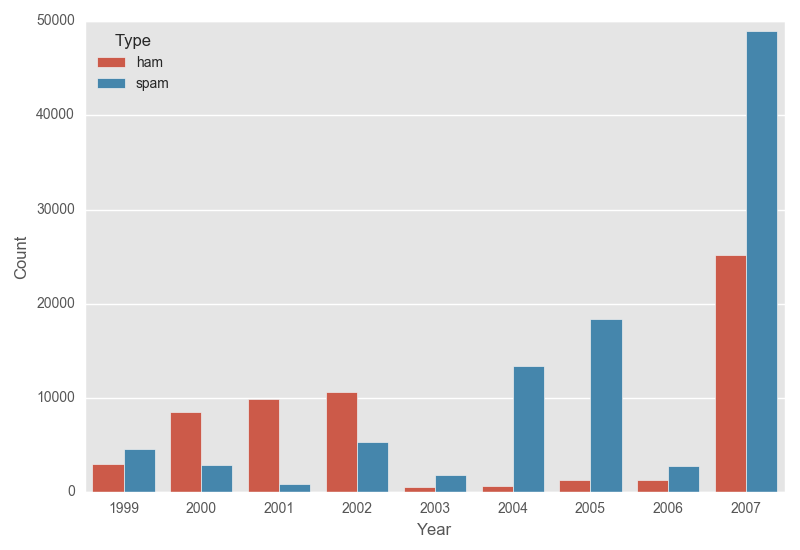
\includegraphics[width=10cm]{Email_count_each_year.png}
\centering
\caption{Amount of Email From 1999 to 2007}
\label{email_every_year}
\end{figure}\\

\begin{table}[h]
\centering
\caption{Proportion of Ham Email and Spam Email From 1999 to 2007}
\label{proportion_ham_spam}
\begin{tabular}{@{}llllll@{}}
\toprule
Year & Ham   & Spam  & Ham \%   & Spam \%  & Total \\ \midrule
1999 & 2978  & 4611  & 0.392410 & 0.607590 & 7589  \\
2000 & 8512  & 2851  & 0.749098 & 0.250902 & 11363 \\
2001 & 9872  & 848   & 0.920896 & 0.079104 & 10720 \\
2002 & 10663 & 5280  & 0.668820 & 0.331180 & 15943 \\
2003 & 545   & 1773  & 0.235116 & 0.764884 & 2318  \\
2004 & 627   & 13420 & 0.044636 & 0.955364 & 14047 \\
2005 & 1309  & 18418 & 0.066356 & 0.933644 & 19727 \\
2006 & 1226  & 2730  & 0.309909 & 0.690091 & 3956  \\
2007 & 25219 & 48999 & 0.339796 & 0.660204 & 74218 \\ \bottomrule
\end{tabular}
\end{table}\\

After finishing the data cleaning up, we delete the emails with year not between 1999 to 2007 to prevent the situation that the date of the emails is after when the data was collected and that the date of email is so early that the email are still not common used. There are 159981 email with 60951 of them are ham and the other 98930 are spam. From Table \ref{proportion_ham_spam} and Figure \ref{email_every_year}, we can see that there is a disproportional number of emails between each year as well as between spam and ham groups. The imbalance dataset may be worrisome for our classifiers. However, there is not much we can do about this situation. Maybe if we can see that there is not too much variation between ham and spam emails across years or there is no time obvious time effect on the emails, then combining the different years wouldn't be a problem. To see whether there are differences in email across the email, we will examine the top words by year. Figure \ref{email_hour_weekday} shown the amount of the email sent each hour and each day. There is a peak for sending spam email at around 12:00 to 15:00. However, ham emails were usually sent between 8:00 to 20:00. Also, according to the right plot of Figure \ref{email_hour_weekday}, ham emails tend to be sent during weekdays and has lower proportion in weekend but spam email seems to be balance each day.\\


\begin{figure}[H]
\begin{subfigure}{\textwidth}
  \centering
  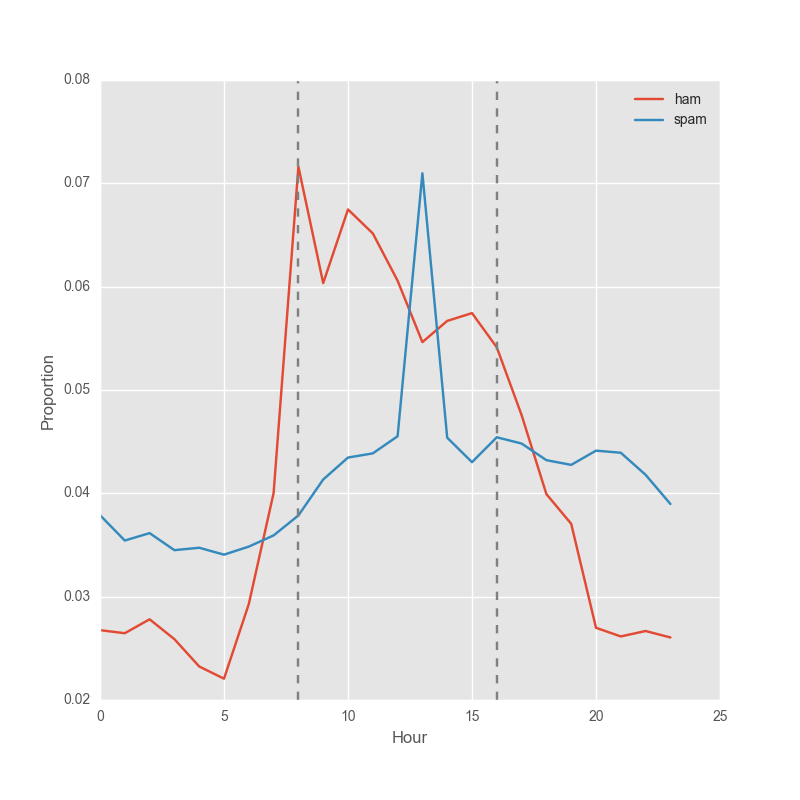
\includegraphics[width=.4\linewidth]{Ham_and_Spam_per_hour.png}
  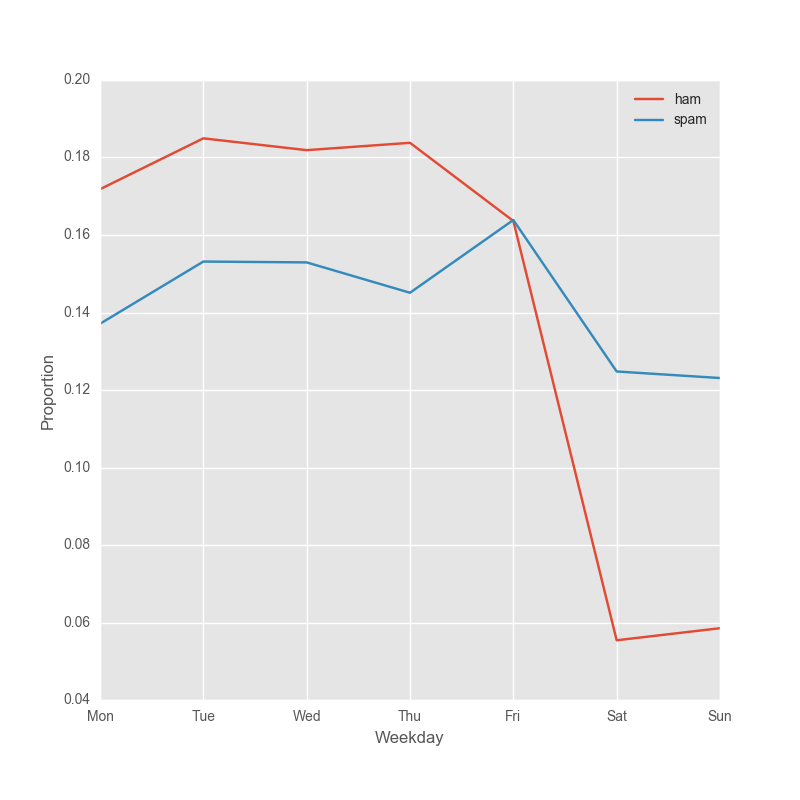
\includegraphics[width=.4\linewidth]{Ham_and_Spam_weekday.png}\\
\end{subfigure}%
\caption{Amount of Email Hourly and On Different Weekday}
\label{email_hour_weekday}
\end{figure}

\subsection{Top 10 Words Per Year}

% !TEX root = main.tex

One of the main purposes for this project is to explore whether the keywords for spam and ham email changed by year. In this section, we counted the appear frequency of each word as a vector by year respectively. Sort the frequency and find out the top 10 frequent words per year. We would like to explore that whether the frequent words changed by year. Moreover, in the next section, we will use word cloud to visualize the results we found out.\\

According to the Figure.\ref{topwordspam}, although keywords did not change year by year, we still have found out that there might have a difference in 2002. Before 2001, some keywords appreared repeatedly, such as "microsoft", "adobe", "windows", and "free". It seems before 2001, in our data set, the spam emails mostly are related to computer and Microsoft topics. From 2002, "stock", "business", "money", and  "com" become top frequent keywords. We categorize those as economy and Internet topics. \\

For the ham email (Figure. \ref{topwordham}), there is not specific topic for each year. We cannot conclude any specific topic or gap for year. However, overall keywords mainly focus on acadmic, such as "edu", "university", "data". We inferred that ham email data may mostly come from academic organizations.\\

\begin{figure}[H]
    \centering
    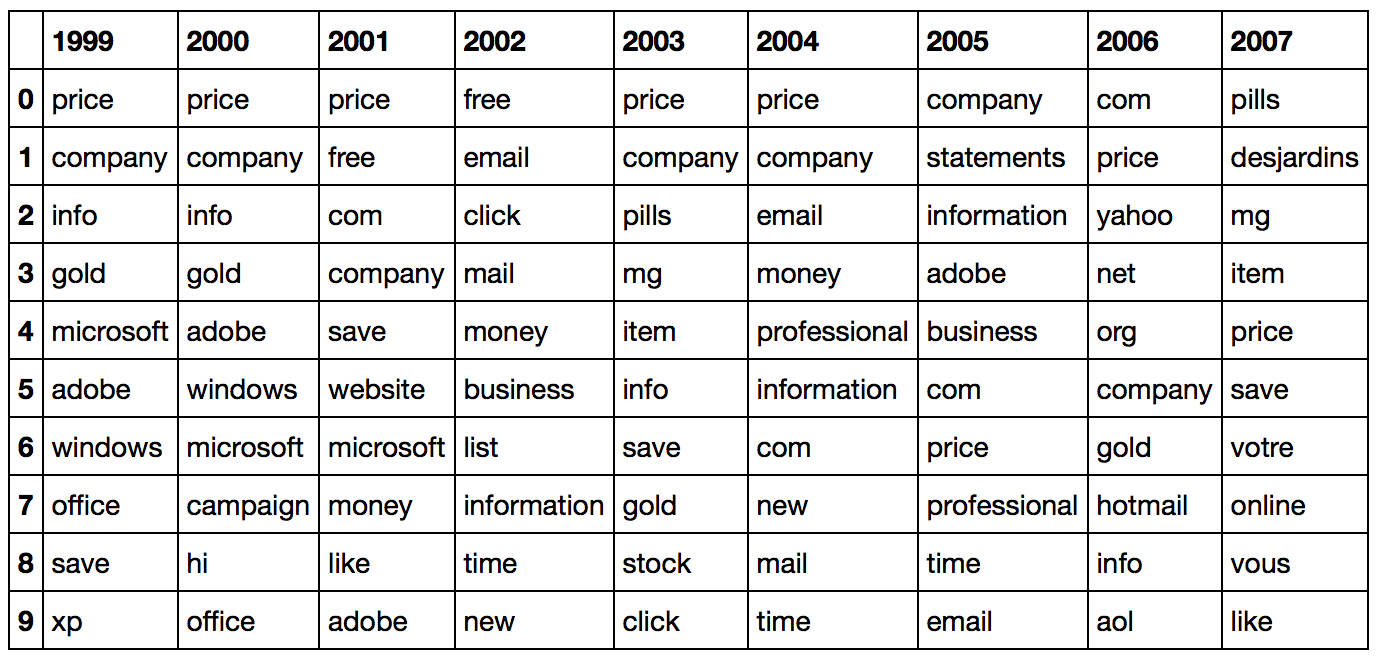
\includegraphics[width=13cm]{./plots/top_word_spam.png}
    \caption{Top 10 Frequent Words Of Spam Email}
    \label{topwordspam}
\end{figure}


\begin{figure}[H]
    \centering
    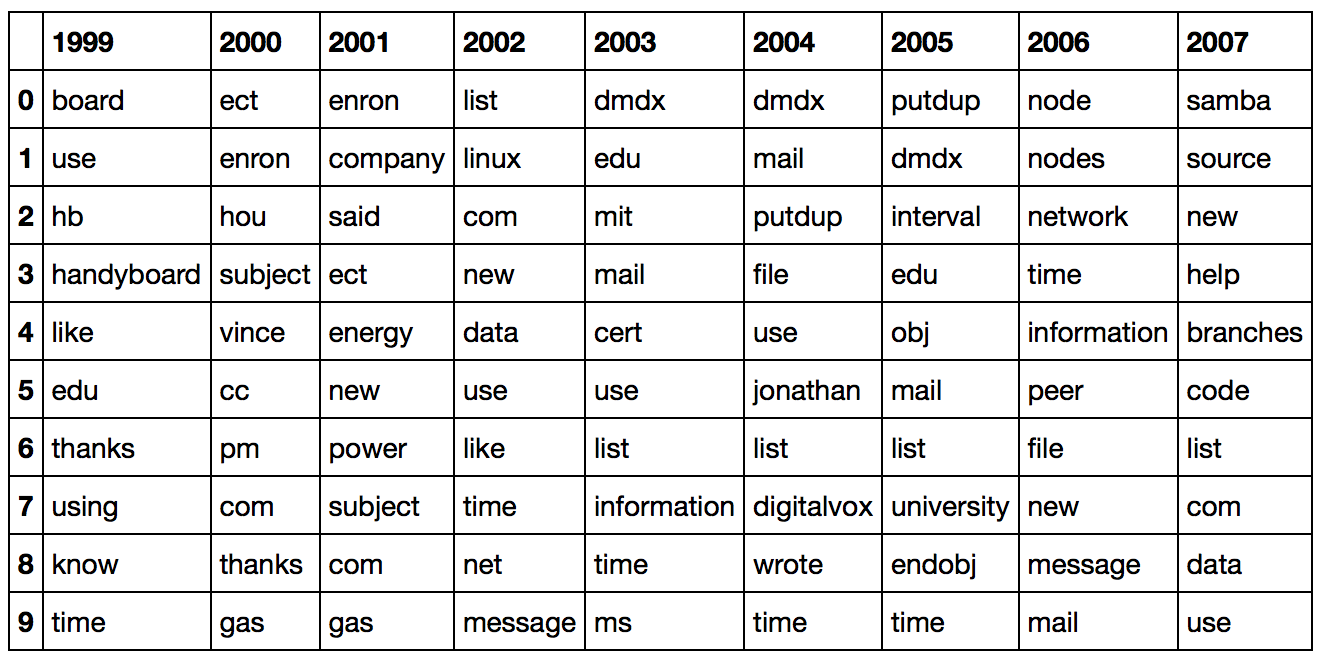
\includegraphics[width=13cm]{./plots/top_word_ham.png}
    \caption{Top 10 Frequent Words Of Ham Email}
    \label{topwordham}
\end{figure}




\subsection{Word Cloud}

% !TEX root = main.tex
\vskip -2ex

\begin{figure}[H]
\begin{subfigure}{\textwidth}
  \centering
  \includegraphics[width=.4\linewidth]{{"./plots/wordCloudImages/Ham 1999"}.png}
  \includegraphics[width=.4\linewidth]{{"./plots/wordCloudImages/Spam 1999"}.png} \\
  
   \vskip -7ex
   
   \includegraphics[width=.4\linewidth]{{"./plots/wordCloudImages/Ham 2000"}.png}
  \includegraphics[width=.4\linewidth]{{"./plots/wordCloudImages/Spam 2000"}.png} \\
  
  \vskip -7ex
    
  \includegraphics[width=.4\linewidth]{{"./plots/wordCloudImages/Ham 2001"}.png}
  \includegraphics[width=.4\linewidth]{{"./plots/wordCloudImages/Spam 2001"}.png} \\ 
  
  \vskip -7ex
  
   \includegraphics[width=.4\linewidth]{{"./plots/wordCloudImages/Ham 2002"}.png}
  \includegraphics[width=.4\linewidth]{{"./plots/wordCloudImages/Spam 2002"}.png} \\ 
  
  \vskip -7ex
  
    \includegraphics[width=.4\linewidth]{{"./plots/wordCloudImages/Ham 2003"}.png}
  \includegraphics[width=.4\linewidth]{{"./plots/wordCloudImages/Spam 2003"}.png} \\ 
  
  \vskip -7ex
  
  \includegraphics[width=.4\linewidth]{{"./plots/wordCloudImages/Ham 2004"}.png}
  \includegraphics[width=.4\linewidth]{{"./plots/wordCloudImages/Spam 2004"}.png} \\   
  
\end{subfigure}%
\caption{Word Cloud For Spam And Ham Email From 1999 to 2004}
\end{figure}

\begin{figure}[H]
\begin{subfigure}{\textwidth}
\centering
  
  \includegraphics[width=.4\linewidth]{{"./plots/wordCloudImages/Ham 2005"}.png}
  \includegraphics[width=.4\linewidth]{{"./plots/wordCloudImages/Spam 2005"}.png} \\ 
  
  \vskip -7ex
  
  \includegraphics[width=.4\linewidth]{{"./plots/wordCloudImages/Ham 2006"}.png}
  \includegraphics[width=.4\linewidth]{{"./plots/wordCloudImages/Spam 2006"}.png} \\ 
  
  \vskip -7ex
  
  \includegraphics[width=.4\linewidth]{{"./plots/wordCloudImages/Ham 2007"}.png}
  \includegraphics[width=.4\linewidth]{{"./plots/wordCloudImages/Spam 2007"}.png} 
  
\end{subfigure}%
\caption{Word Cloud For Spam And Ham Email From 2005 to 2007}
\end{figure}

From the wordclouds, we see that Microsoft and windows XP seem to be a consistent theme in spam. However, we do see a shift less on windows and more towards sales and products during the later half. For ham, based on the words that show up, we may think that the email data originate from an education or technical source due to terms like edu and systems. \\

\section{Previous Studies}
\documentclass[10pt, letterpaper, titlepage]{article}
\usepackage{graphicx}
\usepackage{enumerate}
\begin{document}


\textbf{Introduction}\\
It is important to study what people did and create our study on top of it. In this section, we focus on summarize previous studies of spam/ham e-mail filtering and their machine learning methods. At the end of this section, we point out the new methods and new data we use in this project to show our understanding.  \\

\textbf{Previous Studies}\\
People already came up with the idea of spam/ham e-mail filtering before 2004. In the paper \textit{Machine Learning Techniques in Spam Filtering} written by Konstantin in 2004, the experiment used four main methods : Naive Bayes, K-NN, Perceptron, and SVM. And compare accuracy rate of each methods. In this basic practice, they found the Perceptron method has the highest accuracy rate, 98.5\% with a corpus of 1099 messages. \\

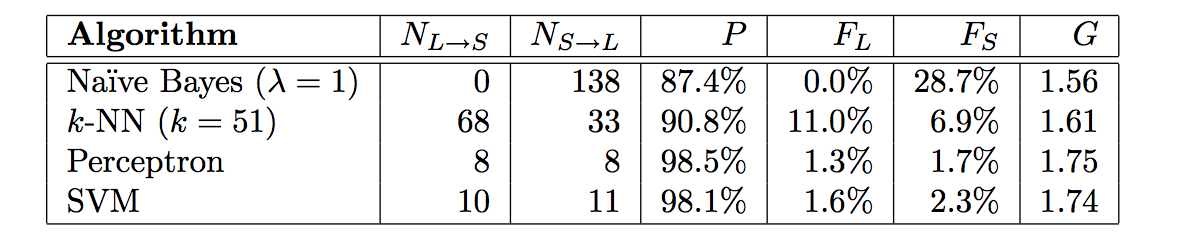
\includegraphics[scale=1.0, width=\linewidth]{2004.png}\\

In 2010, \textit{Email Spam Filtering using Supervised Machine Learning Techniques } written by V.Christina, they used Naive Bayes, J-48(Decision Tree) and Multilayer Perceptron. And they found out MLP performed the best with 99.3\% accuracy rate when experimenting with a corpus of 1500 messages.\\

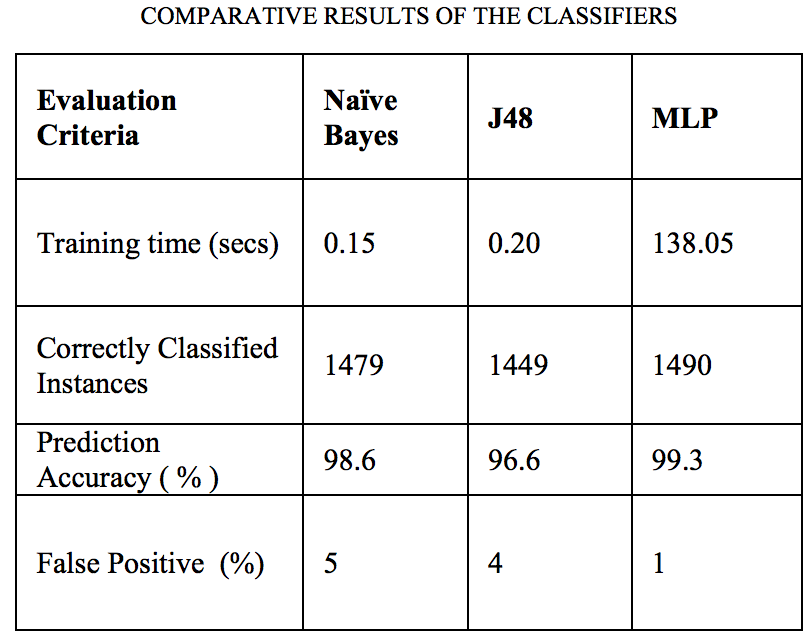
\includegraphics[width=5.5cm,height=5cm,keepaspectratio]{2010-1.png}
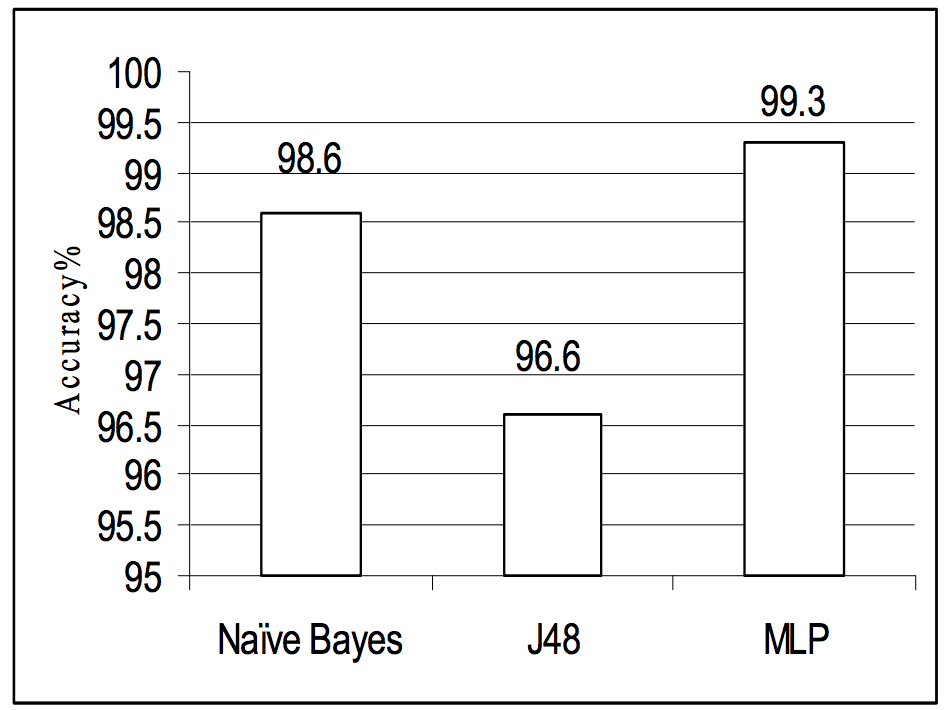
\includegraphics[width=5.5cm,height=5cm,keepaspectratio]{2010-2.png}

In 2016, \textit{Spam Mail Detection using Classification} written by Parhat and Gambhir used Naive Bayes, SVM and J-48(Decision Tree). And they found out Naive Bayes performed the best with 76\% accuracy rate in their experiment. \\ And \textit{Email Spam Detection} written by Ge and  Lauren, used the corpus from TREC 2007 with 1000 messages. They tried logistic regression, Naive Bayesian, Decision Tree and K-NN. The finally found KNN with highest 99\% accuracy rate. \\
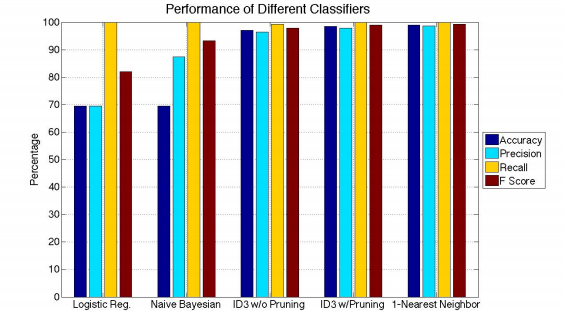
\includegraphics[width=10cm,height=5cm,keepaspectratio]{2016.png}

Here is the summary of methods in each previous studies by year. 

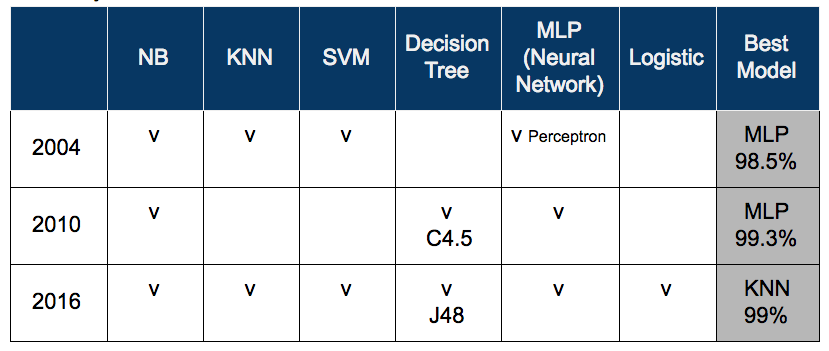
\includegraphics[width=10cm,height=10cm,keepaspectratio]{Method_Summary.png}\\


\textbf{Our works}\\

\begin{enumerate}
	\item \textbf{Use multiple data source}: In each paper, they mainly use a single year of corpus data. In our project, we tried to source different e-mail and integrate them. The format of each data source is different thus hard to clean. And we successfully got to manage a huge data set. 
	\item \textbf{Try 6 methods at the same time}: Previous studies compare accuracy rate with different methods, but they didn't compare them all at a time. So we studied the methods from 2004 to 2016, and apply all of possible methods with adequate tuning parameters to compare them 
	\item \textbf{Apply 1-Gram and 2-Gram}: Each paper marked that data processing step is important to a good result. Here, we introduced bag of words of 1-Gram and 2-Gram methods in the feature engineering part. And we can see different result of accuracy rate in the following section.
\end{enumerate}

\end{document}

\section{Method}

\subsection{Feature Engineering}
First all of, we decoded and encoded the email content to ascii. Then we generalized the notion of word to every basic unit of characters based on whitespace and made all of characters as a list. This process is called tokenization. After creating the list of texts, we remove the stop word to reduce the noise from contents. In addition to create the list of unit characters, we also tried bag of n-grams models for unit-gram and bi-gram to count the frequency of words.\\

After having previous step, we used tf-idf to give weight of words in each email. Total number of 1-gram bag of words in training data is 1053414. We would use this tf-idf model to fit the testing data.\\ Because the total number of email data we have is 111916. The number of word features is much larger than the data we have. In this case, the number of features(p) is larger than the number of data set(n). Therefore, we need to do the data reduction.\\

The method we used for data reduction is called Latent Semantic Analysis (LSA) which is similar with Singular Value Decomposition (SVD). LSA can help us reduce the number of features without losing too much information. LSA also used the consine of the angle between two vectors to form the feature matrix. We reduced our features to only 100 dimensions and used reduced features matrix to fit the models.

In the Figure. \ref{fig:FE}, we displayed the scatter plot of first two components. We can find out that the spam and ham email have been lightly separated.

\begin{figure}[ht!]
    \centering
    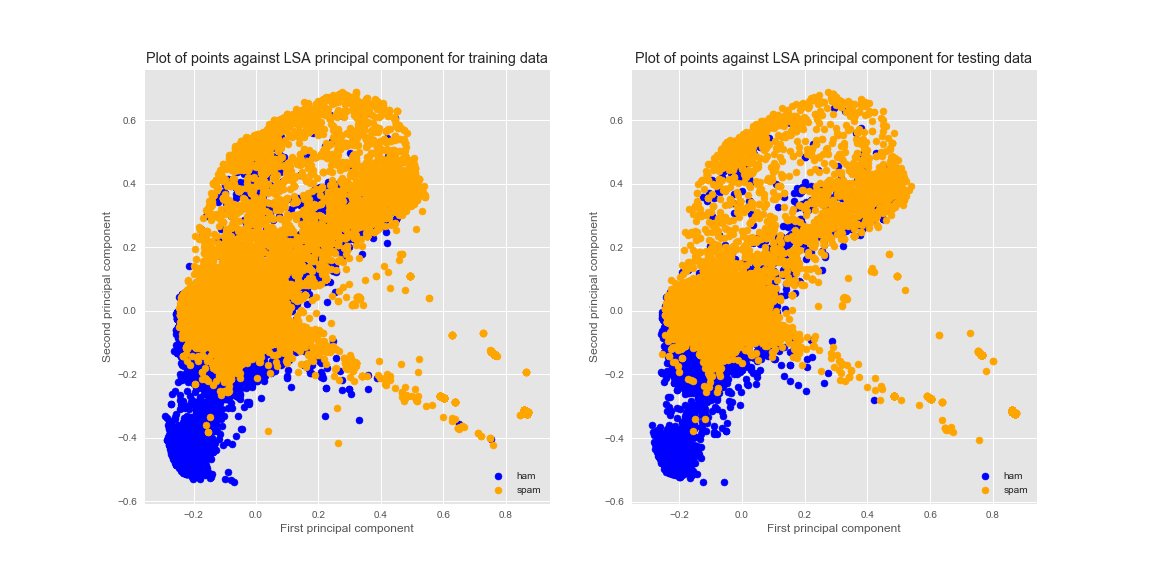
\includegraphics[scale=0.4]{data_reduction_cp12.png}
    \caption{Latent Semantic Analysis Components Plots}
    \label{fig:FE}
\end{figure}



\pagebreak

\subsection{Fit Models}
\subsubsection{Navie Bayes}
\textbf{Naive Bayes}\\
Naive Bayes has a very strong assumption that components of the vector x are independent in each class. However, in this data set, we may easily think of the situation that words are related to each other. So in this case, we will not expect Naive Bayes to perform better than other methods. And we found out that the accuracy rate of Naive Bayes has the lowest accuracy rate: 0.7304 for 1-gram and 0.7281 for 2-gram. 

\begin{table}[H]
	\begin{floatrow}
		\capbtabbox{  
			\begin{subtable}{.45\textwidth}
				\centering
				\begin{tabular}{@{}|c|c|c|c|@{}}
					\toprule
					\multicolumn{2}{|c|}{\multirow{2}{*}{Unit-gram}} & \multicolumn{2}{c|}{Actual} \\ \cmidrule(l){3-4} 
					\multicolumn{2}{|c|}{}                        & Ham          & Spam         \\ \midrule
					\multirow{2}{*}{Predicted}       & Ham        & 15123        & 9877         \\ \cmidrule(l){2-4} 
					& Spam       & 3054         & 19919        \\ \bottomrule
				\end{tabular}
				
				\begin{tabular}{@{}|c|c|c|c|@{}}
					\toprule
					\multicolumn{2}{|c|}{\multirow{2}{*}{Bi-gram}} & \multicolumn{2}{c|}{Actual} \\ \cmidrule(l){3-4} 
					\multicolumn{2}{|c|}{}                        & Ham          & Spam         \\ \midrule
					\multirow{2}{*}{Predicted}       & Ham        & 14905        & 9624         \\ \cmidrule(l){2-4} 
					& Spam       & 3416         & 20020        \\ \bottomrule
				\end{tabular}
			\end{subtable}
		}{  
			\caption{Confusion Matrix with Naive Bayes}  
			\label{Confusion_NB}  
		}  
		\capbtabbox{  
			\begin{subtable}{.5\textwidth}
				\centering
				\begin{tabular}{@{}|c|c|c|c|@{}}
					\toprule
					\multicolumn{2}{|c|}{\multirow{2}{*}{Unit-gram}} & \multicolumn{2}{c|}{Actual} \\ \cmidrule(l){3-4} 
					\multicolumn{2}{|c|}{}                        & Ham          & Spam         \\ \midrule
					\multirow{2}{*}{Predicted}       & Ham        & 16837        & 1167         \\ \cmidrule(l){2-4} 
					& Spam       & 1484         & 28477        \\ \bottomrule
				\end{tabular}
				
				\begin{tabular}{@{}|c|c|c|c|@{}}
					\toprule
					\multicolumn{2}{|c|}{\multirow{2}{*}{Bi-gram}} & \multicolumn{2}{c|}{Actual} \\ \cmidrule(l){3-4} 
					\multicolumn{2}{|c|}{}                        & Ham          & Spam         \\ \midrule
					\multirow{2}{*}{Predicted}       & Ham        & 16787        & 1353         \\ \cmidrule(l){2-4} 
					& Spam       & 1534         & 28291        \\ \bottomrule
				\end{tabular}
			\end{subtable}
		}{  
			\caption{Confusion Matrix For Decision Tree}  
			\label{Confusion_DT}  
		}  
	\end{floatrow}
\end{table} 


\subsubsection{Decision Tree}
For decision tree, we use cross validation to tune the parameter max\_depth which represent the maximum depth of the tree. The candidate of the parameter is the 10, 20, 50, and the default one which is that the nodes are expanded until all leaves are pure or until all leaves contain less than min\_samples\_split samples. When tuning the model fitting with unit-gram tfidf after data reduction, the average running time for each is around 80 seconds while when max\_depth is 10, the running time would be the shortest. The best parameter is max\_depth=20 with its corresponding accuracy rate 0.9447. The confusion matrix is shown in Table \ref{Confusion_DT}. When the data original is ham email, we will mis-classificated it to be spam email 8.1\% of the time. While when the data is a spam email, we will mis-classificated it to be ham email 3.9367\% of time. This implies that for a ham email, we will have higher probability to have wrong prediction.\\

If right now we change to use bi-gram tfidf to fit the models with the same candidate of parameters, the time for fitting a model will be much longer than fitting unit-gram. It's around 1300 seconds to fit a model. The best parameter here is also max\_depth = 20. The accuracy rate here is 0.9398, which is smaller than that of one-gram model with max\_depth = 20. The confusion matrix is shown in Table \ref{Confusion_DT}. The mis-classification rate when the data is ham will be 8.3729\% and that for a spam email is 4.5641\%. The ham email will also have higher probability to predict wrong. 


\begin{table}[H]
\centering
\begin{subtable}{.5\textwidth}
\centering
\begin{tabular}{@{}|c|c|c|c|@{}}
\toprule
\multicolumn{2}{|c|}{\multirow{2}{*}{Unit-gram}} & \multicolumn{2}{c|}{Actual} \\ \cmidrule(l){3-4} 
\multicolumn{2}{|c|}{}                        & Ham          & Spam         \\ \midrule
\multirow{2}{*}{Predicted}       & Ham        & 16837        & 1167         \\ \cmidrule(l){2-4} 
                                 & Spam       & 1484         & 28477        \\ \bottomrule
\end{tabular}

\begin{tabular}{@{}|c|c|c|c|@{}}
\toprule
\multicolumn{2}{|c|}{\multirow{2}{*}{Bi-gram}} & \multicolumn{2}{c|}{Actual} \\ \cmidrule(l){3-4} 
\multicolumn{2}{|c|}{}                        & Ham          & Spam         \\ \midrule
\multirow{2}{*}{Predicted}       & Ham        & 16787        & 1353         \\ \cmidrule(l){2-4} 
                                 & Spam       & 1534         & 28291        \\ \bottomrule
\end{tabular}
\end{subtable}
\caption{Confusion Matrix For Decision Tree With One-gram And Bi-gram TFIDF}
\label{Confusion_DT}
\end{table}


\subsubsection{SVMs}
We would like to use two SVM methods: Linear and RBF to do the classification. Because of the size of data, it is not easy to tune cross-validation. Therefore, we decide to use the 3-folder cross validation as our standard then tune the penalty parameter of the error term.The number of penalty parameter we chose for tuning is : 0.001,0.01,0.05,0.1,0.2,0.5,0.7, and 1.\\
After tuning the penalty parameter, the result from test data indicated taht accuracy rate in Linear SVM performs better than RBF SMV. For the uni-gram and bi-gram, Linear SVM has similar accuracy rate. However, RBF SVM has higher accuracy in uni-gram. About the confusion matrix, the prediction of spam/ham email has similar error rate in each method. \\
The weakness of SVM is that tuning the parameters and fitting the model is time consuming. In practice, costing too much time to predict results may increase the cost on industry especially when the data set is large. Therefore, we thought in the SVMs, time will be particularly noteworthy.

\begin{table*}
\begin{floatrow}
\capbtabbox{  
 \begin{subtable}{.45\textwidth}
\centering
\begin{tabular}{@{}|c|c|c|c|@{}}
\toprule
\multicolumn{2}{|c|}{\multirow{2}{*}{Unit-gram}} & \multicolumn{2}{c|}{Actual} \\ \cmidrule(l){3-4} 
\multicolumn{2}{|c|}{}                        & Ham          & Spam         \\ \midrule
\multirow{2}{*}{Predicted}       & Ham        & 16667        & 944         \\ \cmidrule(l){2-4} 
                                 & Spam       & 1654         & 28700        \\ \bottomrule
\end{tabular}

\begin{tabular}{@{}|c|c|c|c|@{}}
\toprule
\multicolumn{2}{|c|}{\multirow{2}{*}{Bi-gram}} & \multicolumn{2}{c|}{Actual} \\ \cmidrule(l){3-4} 
\multicolumn{2}{|c|}{}                        & Ham          & Spam         \\ \midrule
\multirow{2}{*}{Predicted}       & Ham        & 16730        & 998         \\ \cmidrule(l){2-4} 
                                 & Spam       & 1591         & 28646        \\ \bottomrule
\end{tabular}
\end{subtable}
}{  
 \caption{Confusion Matrix with Linear SVM}  
 \label{tab:cflinsv}  
}  
\capbtabbox{  
 \begin{subtable}{.45\textwidth}
\centering
\begin{tabular}{@{}|c|c|c|c|@{}}
\toprule
\multicolumn{2}{|c|}{\multirow{2}{*}{Unit-gram}} & \multicolumn{2}{c|}{Actual} \\ \cmidrule(l){3-4} 
\multicolumn{2}{|c|}{}                        & Ham          & Spam         \\ \midrule
\multirow{2}{*}{Predicted}       & Ham        & 15303        &  701         \\ \cmidrule(l){2-4} 
                                 & Spam       & 3018         & 28943        \\ \bottomrule
\end{tabular}
\begin{tabular}{@{}|c|c|c|c|@{}}
\toprule
\multicolumn{2}{|c|}{\multirow{2}{*}{Bi-gram}} & \multicolumn{2}{c|}{Actual} \\ \cmidrule(l){3-4} 
\multicolumn{2}{|c|}{}                        & Ham          & Spam         \\ \midrule
\multirow{2}{*}{Predicted}       & Ham        & 14628        & 658         \\ \cmidrule(l){2-4} 
                                 & Spam       & 3693         & 28986        \\ \bottomrule
\end{tabular}
\end{subtable}
}{  
 \caption{Confusion Matrix with RBF SVM}  
 \label{tab:cfrbf}  
}  
\end{floatrow} 

\end{table*}  

\subsubsection{MLP}

\subsubsection{KNN}
% !TEX root = main.tex

When fitting KNN models, we tuned the parameters with three candidate of K including 3, 5, and 7. The running time is much longer comparing to decision tree. For uni-gram tfidf, the running time for predicting testing data is 457, 441, 494 for each K respectively. After tuning the parameter, the best K for uni-gram tfidf is K=3. The accuracy rate is 0.9657. When using bi-gram tfidf to fit the models, the best K is also 3 with the accuracy rate 0.9678. Using bi-gram in KNN model will improve our prediction. Table \ref{Confusion_KNN} showed the confusion matrix of KNN model with both uni-gram and bi-gram tfidf. Comparing the mis-classification rate for each class, when the observations are ham email, we will have high probability to have wrong prediction.\\



\begin{table}[H]
				\centering
	\begin{floatrow}
		\capbtabbox{  
			\begin{subtable}{.5\textwidth}

			\begin{tabular}{@{}|c|c|c|c|@{}}
				\toprule
				\multicolumn{2}{|c|}{\multirow{2}{*}{Unit-gram}} & \multicolumn{2}{c|}{Actual} \\ \cmidrule(l){3-4} 
				\multicolumn{2}{|c|}{}                        & Ham          & Spam         \\ \midrule
				\multirow{2}{*}{Predicted}       & Ham        & 17331        & 651          \\ \cmidrule(l){2-4} 
				& Spam       & 990          & 28993        \\ \bottomrule
			\end{tabular}
			\begin{tabular}{@{}|c|c|c|c|@{}}
				\toprule
				\multicolumn{2}{|c|}{\multirow{2}{*}{Bi-gram}} & \multicolumn{2}{c|}{Actual} \\ \cmidrule(l){3-4} 
				\multicolumn{2}{|c|}{}                        & Ham          & Spam         \\ \midrule
				\multirow{2}{*}{Predicted}       & Ham        & 17405        & 626          \\ \cmidrule(l){2-4} 
				& Spam       & 916          & 29018        \\ \bottomrule
			\end{tabular}
		\end{subtable}
		}{  
			\caption{Confusion Matrix For KNN}  
			\label{Confusion_KNN}  
		}  
		\capbtabbox{  
			\begin{subtable}{.5\textwidth}
				\centering
				\begin{tabular}{@{}|c|c|c|c|@{}}
					\toprule
					\multicolumn{2}{|c|}{\multirow{2}{*}{Unit-gram}} & \multicolumn{2}{c|}{Actual} \\ \cmidrule(l){3-4} 
					\multicolumn{2}{|c|}{}                        & Ham          & Spam         \\ \midrule
					\multirow{2}{*}{Predicted}       & Ham        & 16343       & 1375          \\ \cmidrule(l){2-4} 
					& Spam       & 1834          & 28413        \\ \bottomrule
				\end{tabular}
				\begin{tabular}{@{}|c|c|c|c|@{}}
					\toprule
					\multicolumn{2}{|c|}{\multirow{2}{*}{Bi-gram}} & \multicolumn{2}{c|}{Actual} \\ \cmidrule(l){3-4} 
					\multicolumn{2}{|c|}{}                        & Ham          & Spam         \\ \midrule
					\multirow{2}{*}{Predicted}       & Ham        & 16705        & 1336          \\ \cmidrule(l){2-4} 
					& Spam       & 1616          & 28308        \\ \bottomrule
				\end{tabular}
			\end{subtable}
		}{  
			\caption{Confusion Matrix For Logistic}  
			\label{Confusion_Logistic}  
		}  
	\end{floatrow}
\end{table} 




\subsubsection{Logistic}
% !TEX root = main.tex

Here we first trained the logistic parameters. We found out that uni-gram tfidf has the maximum accuracy rate with C = 7 (or 8) and the accuracy rate of bi-gram converges when C goes larger. Therefore, we set C= 199. By running approximately 1000 secs, we got accuracy rate of 0.9331 for uni-gram and 0.9384 for bi-gram. This is a method with decent running time (cost) and good accuracy rate. \\

\section{Conclusion and exploration}


\begin{table}[H]
	\centering
	\caption{Summary of Models Using Unit-Gram}
	\label{Summary-one-gram}
	\begin{tabular}{lccccccc}
		\hline
		Model      & Logistic             & Naive Bayes          & KNN                     & Decision Tree & MLP                  & Linear SVM & rbf SVM \\ \hline
		Accuracy   &                      &                      & 0.9658                  & 0.9447        &                      & 0.9458     & 0.92246 \\
		Time (sec) & \multicolumn{1}{l}{} & \multicolumn{1}{l}{} & \multicolumn{1}{l}{457} & 81.1206       & \multicolumn{1}{l}{} & 6504       & 4024    \\ \hline
	\end{tabular}
\end{table}


\begin{table}[H]
	\centering
	\caption{Summary of Models Using Bi-Gram}
	\label{Summary-bi-gram}
	\begin{tabular}{lccccccc}
		\hline
		Model      & Logistic & Naive Bayes & KNN    & Decision Tree & MLP & Linear SVM & rbf SVM \\ \hline
		Accuracy   &          &             & 0.9678 & 0.9398        &     & 0.9460     & 0.9093  \\
		Time (sec) &          &             & 1107   & 1220.9498     &     & 16802      & 144056  \\ \hline
	\end{tabular}
\end{table}

\section{Reference}



\end{document}
